\documentclass{standalone}
\usepackage{tikz}
\usetikzlibrary{patterns, positioning}


\begin{document}
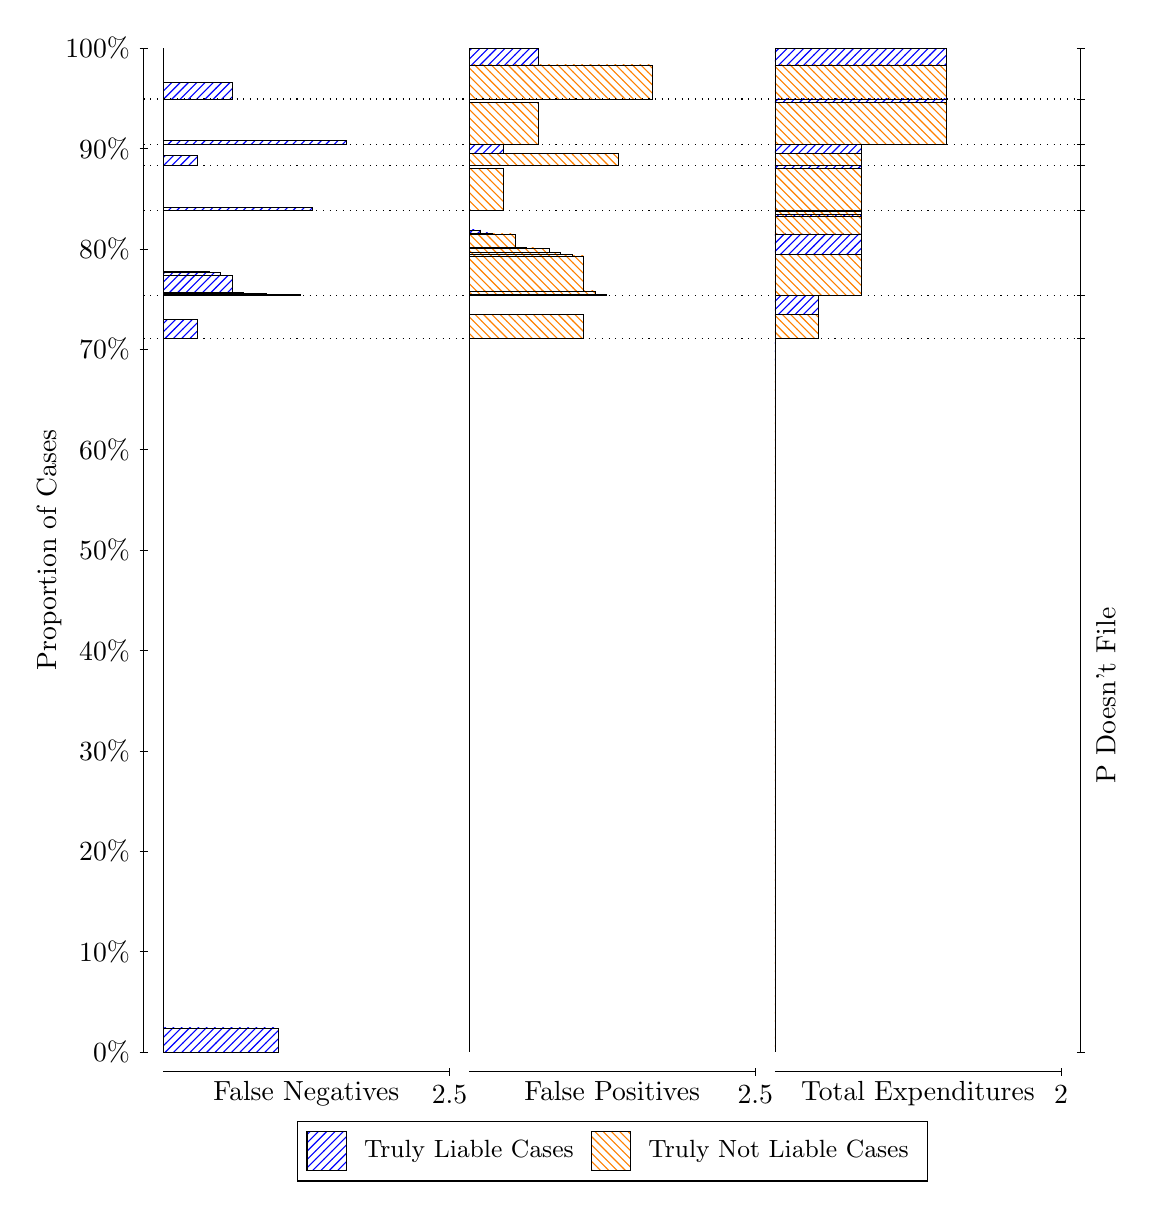
\begin{tikzpicture}
\draw[black, very thin] (1.5,1.75) -- (1.5,14.5);
\node[rotate=90, text=black, anchor=center] at (0.3, 8.125) {Proportion of Cases};
\draw[black, very thin] (1.45,1.75) -- (1.55,1.75);
\node[text=black, anchor=east] at (1.45, 1.75) {0\%};
\draw[black, very thin] (1.45,3.025) -- (1.55,3.025);
\node[text=black, anchor=east] at (1.45, 3.025) {10\%};
\draw[black, very thin] (1.45,4.3) -- (1.55,4.3);
\node[text=black, anchor=east] at (1.45, 4.3) {20\%};
\draw[black, very thin] (1.45,5.575) -- (1.55,5.575);
\node[text=black, anchor=east] at (1.45, 5.575) {30\%};
\draw[black, very thin] (1.45,6.85) -- (1.55,6.85);
\node[text=black, anchor=east] at (1.45, 6.85) {40\%};
\draw[black, very thin] (1.45,8.125) -- (1.55,8.125);
\node[text=black, anchor=east] at (1.45, 8.125) {50\%};
\draw[black, very thin] (1.45,9.4) -- (1.55,9.4);
\node[text=black, anchor=east] at (1.45, 9.4) {60\%};
\draw[black, very thin] (1.45,10.675) -- (1.55,10.675);
\node[text=black, anchor=east] at (1.45, 10.675) {70\%};
\draw[black, very thin] (1.45,11.95) -- (1.55,11.95);
\node[text=black, anchor=east] at (1.45, 11.95) {80\%};
\draw[black, very thin] (1.45,13.225) -- (1.55,13.225);
\node[text=black, anchor=east] at (1.45, 13.225) {90\%};
\draw[black, very thin] (1.45,14.5) -- (1.55,14.5);
\node[text=black, anchor=east] at (1.45, 14.5) {100\%};

\draw[black, very thin] (13.4,1.75) -- (13.4,14.5);
\draw[black, very thin] (13.35,1.75) -- (13.45,1.75);
\node[anchor=west] at (13.35, 1.75) {};
\draw[black, very thin] (13.35,10.81) -- (13.45,10.81);
\node[anchor=west] at (13.35, 10.81) {};
\draw[black, very thin] (13.35,11.36) -- (13.45,11.36);
\node[anchor=west] at (13.35, 11.36) {};
\draw[black, very thin] (13.35,12.442) -- (13.45,12.442);
\node[anchor=west] at (13.35, 12.442) {};
\draw[black, very thin] (13.35,13.01) -- (13.45,13.01);
\node[anchor=west] at (13.35, 13.01) {};
\draw[black, very thin] (13.35,13.28) -- (13.45,13.28);
\node[anchor=west] at (13.35, 13.28) {};
\draw[black, very thin] (13.35,13.853) -- (13.45,13.853);
\node[anchor=west] at (13.35, 13.853) {};
\draw[black, very thin] (13.35,14.5) -- (13.45,14.5);
\node[anchor=west] at (13.35, 14.5) {};

\draw[black, very thin, pattern color=blue, pattern=north east lines] (1.75,1.75) rectangle (3.2033,2.0563);
\draw[black, very thin, pattern color=orange, pattern=north west lines] (1.75,2.0563) rectangle (1.75,10.81);
\draw[black, very thin, pattern color=blue, pattern=north east lines] (1.75,10.81) rectangle (2.186,11.056);
\draw[black, very thin, pattern color=orange, pattern=north west lines] (1.75,11.056) rectangle (1.75,11.36);
\draw[black, very thin, pattern color=blue, pattern=north east lines] (1.75,11.36) rectangle (3.494,11.37);
\draw[black, very thin, pattern color=blue, pattern=north east lines] (1.75,11.37) rectangle (3.3487,11.372);
\draw[black, very thin, pattern color=blue, pattern=north east lines] (1.75,11.372) rectangle (3.2033,11.374);
\draw[black, very thin, pattern color=blue, pattern=north east lines] (1.75,11.374) rectangle (3.058,11.382);
\draw[black, very thin, pattern color=blue, pattern=north east lines] (1.75,11.382) rectangle (3.058,11.382);
\draw[black, very thin, pattern color=blue, pattern=north east lines] (1.75,11.382) rectangle (2.9127,11.387);
\draw[black, very thin, pattern color=blue, pattern=north east lines] (1.75,11.387) rectangle (2.7673,11.392);
\draw[black, very thin, pattern color=blue, pattern=north east lines] (1.75,11.392) rectangle (2.622,11.613);
\draw[black, very thin, pattern color=blue, pattern=north east lines] (1.75,11.613) rectangle (2.4767,11.65);
\draw[black, very thin, pattern color=blue, pattern=north east lines] (1.75,11.65) rectangle (2.3313,11.662);
\draw[black, very thin, pattern color=orange, pattern=north west lines] (1.75,11.662) rectangle (1.75,12.442);
\draw[black, very thin, pattern color=blue, pattern=north east lines] (1.75,12.442) rectangle (3.6393,12.479);
\draw[black, very thin, pattern color=orange, pattern=north west lines] (1.75,12.479) rectangle (1.75,13.01);
\draw[black, very thin, pattern color=blue, pattern=north east lines] (1.75,13.01) rectangle (2.186,13.132);
\draw[black, very thin, pattern color=orange, pattern=north west lines] (1.75,13.132) rectangle (1.75,13.28);
\draw[black, very thin, pattern color=blue, pattern=north east lines] (1.75,13.28) rectangle (4.0753,13.327);
\draw[black, very thin, pattern color=orange, pattern=north west lines] (1.75,13.327) rectangle (1.75,13.853);
\draw[black, very thin, pattern color=blue, pattern=north east lines] (1.75,13.853) rectangle (2.622,14.068);
\draw[black, very thin, pattern color=orange, pattern=north west lines] (1.75,14.068) rectangle (1.75,14.5);
\draw[black, very thin, pattern color=orange, pattern=north west lines] (5.6333,1.75) rectangle (5.6333,10.503);
\draw[black, very thin, pattern color=blue, pattern=north east lines] (5.6333,10.503) rectangle (5.6333,10.81);
\draw[black, very thin, pattern color=orange, pattern=north west lines] (5.6333,10.81) rectangle (7.0867,11.114);
\draw[black, very thin, pattern color=blue, pattern=north east lines] (5.6333,11.114) rectangle (5.6333,11.36);
\draw[black, very thin, pattern color=orange, pattern=north west lines] (5.6333,11.36) rectangle (7.3773,11.371);
\draw[black, very thin, pattern color=orange, pattern=north west lines] (5.6333,11.371) rectangle (7.232,11.415);
\draw[black, very thin, pattern color=orange, pattern=north west lines] (5.6333,11.415) rectangle (7.0867,11.861);
\draw[black, very thin, pattern color=orange, pattern=north west lines] (5.6333,11.861) rectangle (6.9413,11.884);
\draw[black, very thin, pattern color=orange, pattern=north west lines] (5.6333,11.884) rectangle (6.796,11.909);
\draw[black, very thin, pattern color=orange, pattern=north west lines] (5.6333,11.909) rectangle (6.6507,11.955);
\draw[black, very thin, pattern color=orange, pattern=north west lines] (5.6333,11.955) rectangle (6.5053,11.962);
\draw[black, very thin, pattern color=orange, pattern=north west lines] (5.6333,11.962) rectangle (6.36,11.968);
\draw[black, very thin, pattern color=orange, pattern=north west lines] (5.6333,11.968) rectangle (6.2147,12.14);
\draw[black, very thin, pattern color=blue, pattern=north east lines] (5.6333,12.14) rectangle (5.924,12.152);
\draw[black, very thin, pattern color=blue, pattern=north east lines] (5.6333,12.152) rectangle (5.7787,12.189);
\draw[black, very thin, pattern color=blue, pattern=north east lines] (5.6333,12.189) rectangle (5.6333,12.442);
\draw[black, very thin, pattern color=orange, pattern=north west lines] (5.6333,12.442) rectangle (6.0693,12.974);
\draw[black, very thin, pattern color=blue, pattern=north east lines] (5.6333,12.974) rectangle (5.6333,13.01);
\draw[black, very thin, pattern color=orange, pattern=north west lines] (5.6333,13.01) rectangle (7.5227,13.158);
\draw[black, very thin, pattern color=blue, pattern=north east lines] (5.6333,13.158) rectangle (6.0693,13.28);
\draw[black, very thin, pattern color=orange, pattern=north west lines] (5.6333,13.28) rectangle (6.5053,13.806);
\draw[black, very thin, pattern color=blue, pattern=north east lines] (5.6333,13.806) rectangle (5.6333,13.853);
\draw[black, very thin, pattern color=orange, pattern=north west lines] (5.6333,13.853) rectangle (7.9587,14.285);
\draw[black, very thin, pattern color=blue, pattern=north east lines] (5.6333,14.285) rectangle (6.5053,14.5);
\draw[black, very thin, pattern color=orange, pattern=north west lines] (9.5167,1.75) rectangle (9.5167,10.503);
\draw[black, very thin, pattern color=blue, pattern=north east lines] (9.5167,10.503) rectangle (9.5167,10.81);
\draw[black, very thin, pattern color=orange, pattern=north west lines] (9.5167,10.81) rectangle (10.062,11.114);
\draw[black, very thin, pattern color=blue, pattern=north east lines] (9.5167,11.114) rectangle (10.062,11.36);
\draw[black, very thin, pattern color=orange, pattern=north west lines] (9.5167,11.36) rectangle (10.607,11.875);
\draw[black, very thin, pattern color=blue, pattern=north east lines] (9.5167,11.875) rectangle (10.607,12.139);
\draw[black, very thin, pattern color=orange, pattern=north west lines] (9.5167,12.139) rectangle (10.607,12.369);
\draw[black, very thin, pattern color=blue, pattern=north east lines] (9.5167,12.369) rectangle (10.607,12.391);
\draw[black, very thin, pattern color=orange, pattern=north west lines] (9.5167,12.391) rectangle (10.607,12.426);
\draw[black, very thin, pattern color=blue, pattern=north east lines] (9.5167,12.426) rectangle (10.607,12.442);
\draw[black, very thin, pattern color=orange, pattern=north west lines] (9.5167,12.442) rectangle (10.607,12.974);
\draw[black, very thin, pattern color=blue, pattern=north east lines] (9.5167,12.974) rectangle (10.607,13.01);
\draw[black, very thin, pattern color=orange, pattern=north west lines] (9.5167,13.01) rectangle (10.607,13.158);
\draw[black, very thin, pattern color=blue, pattern=north east lines] (9.5167,13.158) rectangle (10.607,13.28);
\draw[black, very thin, pattern color=orange, pattern=north west lines] (9.5167,13.28) rectangle (11.697,13.806);
\draw[black, very thin, pattern color=blue, pattern=north east lines] (9.5167,13.806) rectangle (11.697,13.853);
\draw[black, very thin, pattern color=orange, pattern=north west lines] (9.5167,13.853) rectangle (11.697,14.285);
\draw[black, very thin, pattern color=blue, pattern=north east lines] (9.5167,14.285) rectangle (11.697,14.5);
\draw[black, dotted] (1.5,10.81) -- (13.4,10.81);
\draw[black, dotted] (1.5,11.36) -- (13.4,11.36);
\draw[black, dotted] (1.5,12.442) -- (13.4,12.442);
\draw[black, dotted] (1.5,13.01) -- (13.4,13.01);
\draw[black, dotted] (1.5,13.28) -- (13.4,13.28);
\draw[black, dotted] (1.5,13.853) -- (13.4,13.853);
\draw[black, very thin] (1.75,1.5) -- (5.3833,1.5);
\node[text=black, anchor=north] at (3.5667, 1.5) {False Negatives};
\draw[black, very thin] (5.3833,1.45) -- (5.3833,1.55);
\node[text=black, anchor=north] at (5.3833, 1.45) {2.5};

\draw[black, very thin] (5.6333,1.5) -- (9.2667,1.5);
\node[text=black, anchor=north] at (7.45, 1.5) {False Positives};
\draw[black, very thin] (9.2667,1.45) -- (9.2667,1.55);
\node[text=black, anchor=north] at (9.2667, 1.45) {2.5};

\draw[black, very thin] (9.5167,1.5) -- (13.15,1.5);
\node[text=black, anchor=north] at (11.333, 1.5) {Total Expenditures};
\draw[black, very thin] (13.15,1.45) -- (13.15,1.55);
\node[text=black, anchor=north] at (13.15, 1.45) {2};

\node[text=black, centered, rotate=90] at (13.72, 6.2798) {P Doesn't File};







\draw (7.449999999999999,1.5) node[draw=none] (baseCoordinate) {};
\begin{scope}[align=center]
        \matrix[scale=0.5, draw=black, below=0.5cm of baseCoordinate, nodes={draw}, column sep=0.1cm]{
            \node[rectangle, draw, minimum width=0.5cm, minimum height=0.5cm, pattern color=blue, pattern=north east lines] {}; &
            \node[draw=none, font=\small, text=black] (B) {Truly Liable Cases}; &
            \node[rectangle, draw, minimum width=0.5cm, minimum height=0.5cm, pattern color=orange, pattern=north west lines] {}; &
            \node[draw=none, font=\small, text=black] (B) {Truly Not Liable Cases}; \\
            };
\end{scope}

\end{tikzpicture}
\end{document}